\documentclass{ximera}

\usepackage{todonotes}

\newcommand{\RR}{\mathbb R}
\renewcommand{\d}{\,d}
\newcommand{\dd}[2][]{\frac{d #1}{d #2}}
\renewcommand{\l}{\ell}
\newcommand{\ddx}{\frac{d}{dx}}
\newcommand{\dfn}{\textbf}
\newcommand{\eval}[1]{\bigg[ #1 \bigg]}
\renewcommand{\epsilon}{\varepsilon}
\newcommand{\p}[1]{\left(#1\right)}
\newcommand{\br}[1]{\left[#1\right]}
\newcommand{\set}[1]{\left\{#1\right\}}


\let\prelim\lim
\renewcommand{\lim}{\displaystyle\prelim}

\colorlet{textColor}{black} 
\colorlet{background}{white}
\colorlet{penColor}{blue!50!black} % Color of a curve in a plot
\colorlet{penColor2}{red!50!black}% Color of a curve in a plot
\colorlet{penColor3}{red!50!blue} % Color of a curve in a plot
\colorlet{penColor4}{green!50!black} % Color of a curve in a plot
\colorlet{penColor5}{orange!80!black} % Color of a curve in a plot
\colorlet{fill1}{blue!50!black!20} % Color of fill in a plot
\colorlet{fill2}{blue!10} % Color of fill in a plot
\colorlet{fillp}{fill1} % Color of positive area
\colorlet{filln}{red!50!black!20} % Color of negative area
\colorlet{gridColor}{gray!50} % Color of grid in a plot


\newcommand{\fullwidth}{}
\newcommand{\normalwidth}{}



%% makes a snazzy t-chart for evaluating functions
\newenvironment{tchart}{\rowcolors{2}{}{background!90!textColor}\array}{\endarray}


\author{Gregory Hartman \and Matthew Carr}
\license{Creative Commons 3.0 By-NC}
\acknowledgement{https://github.com/APEXCalculus}

\begin{document}
\begin{exercise}

\outcome{Calculate limits from a graph (or state that the limit does not exist).}
\outcome{Explain the relationship between one-sided and two-sided limits.}
\outcome{Distinguish between limit values and function values.}
\outcome{Identify when a limit does not exist.}



\tag{limit} 

% BADBAD
% How should I do hints for this?
% Can we have multiple questions 
% within a single question?


% BADBAD DNE answer

Let $f$ be defined on the interval $\left[0,2\right]$, and no where else, whose graph is:
\begin{center}
\noindent\begin{minipage}[t]{.5\linewidth}
 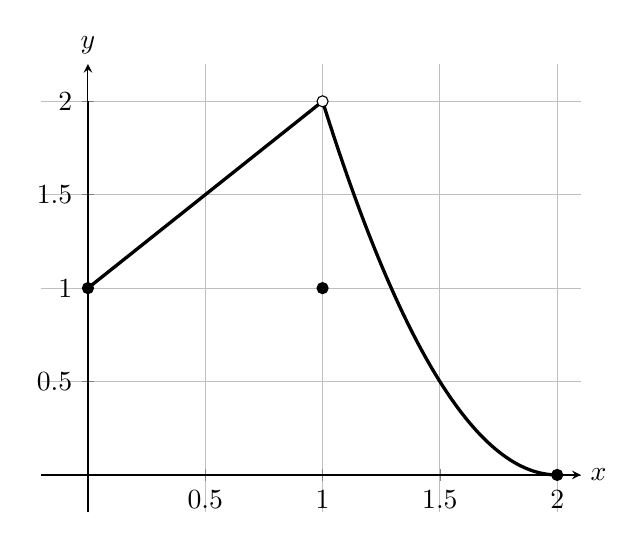
\begin{tikzpicture}
	\begin{axis}
	[ymin=-0.2,ymax=2.2, axis lines=center,xlabel=$x$,ylabel=$y$,every axis y 
	label/.style={at=(current axis.above origin),anchor=south},every axis x label/.style={at=(current axis.right of origin),anchor=west},
	domain=-1:2,
	ytick={0.5,1,1.5,2},
	yticklabels={$0.5$,$1$,$1.5$,$2$},
	xtick={0.5,1.0,1.5,2},
	xticklabels={$0.5$,$1$,$1.5$,$2$},
	ymajorgrids=true,
	grid = major
	]
	\addplot[domain=0:2,very thick,smooth,samples=600]
	{(!(\x>1))*(\x+1)+(\x>1)*(!(\x>2))*(2*(\x-2)^2};
	\addplot[domain=-0.2:2.1, smooth, very thin, samples=100,color=black]
	{0};
	\draw[very thin,color=black] (axis cs:0,-0.2) -- (axis cs:0,2);
	\draw[fill=black] (axis cs:0,1) circle [radius=2pt];
	\draw[fill=black] (axis cs:2,0) circle [radius=2pt];
	\draw[fill=black] (axis cs:1,1) circle [radius=2pt];
	\draw[fill=white] (axis cs:1,2) circle [radius=2pt];
	\end{axis}
       \end{tikzpicture}
\end{minipage}
\end{center}


Find
\noindent\begin{minipage}[t]{.5\linewidth}
\begin{enumerate}
\item		$\lim_{x\to 1^-} f(x)\begin{prompt} = \answer{2}\end{prompt}$
\item		$\lim_{x\to 1^+} f(x)\begin{prompt} = \answer{2}\end{prompt}$
\item		$\lim_{x\to 1} f(x)\begin{prompt} = \answer{2}\end{prompt}$
\end{enumerate}
\end{minipage}
\noindent\begin{minipage}[t]{.5\linewidth}
\begin{enumerate}\addtocounter{enumi}{3}
\item		$f({1})\begin{prompt} = \answer{1}\end{prompt}$
\item		$\lim_{x\to 0^-} f(x)\begin{prompt} = \answer{DNE}\end{prompt}$
\item		$\lim_{x\to 0^+} f(x)\begin{prompt} = \answer{1}\end{prompt}$
\end{enumerate}
\end{minipage}

\end{exercise}
\end{document}